\chapter{Supplementary Experimental Displays}
\label{app:results-supplement}

This appendix retains the predetermined all-input overview and the full
source-level structural descriptions. The main results contain the other
three predetermined plots: ratios by length and the two split-related panels.
Only the main-text histogram is an additional plot. All observations come
from the same complete formal attempt and its qualification evidence.

\begin{figure}[H]
\centering
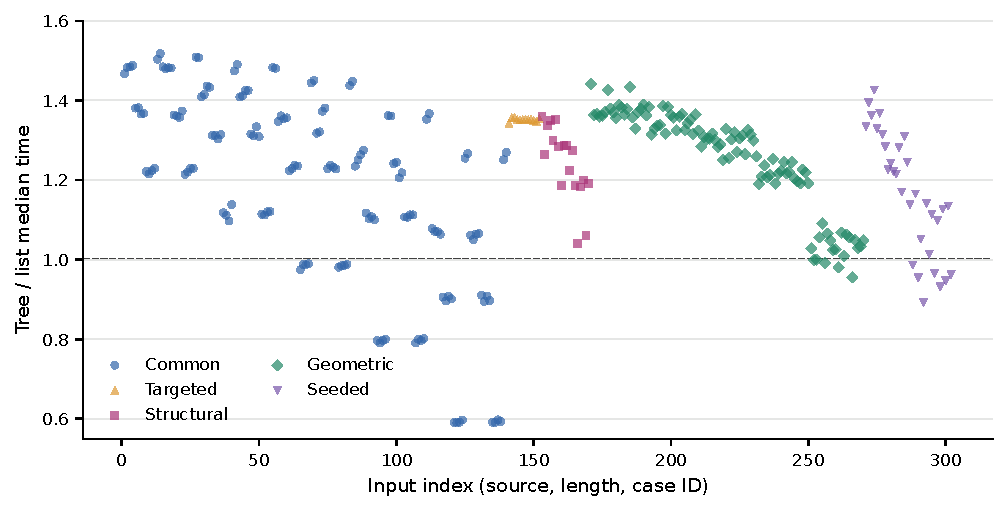
\includegraphics[width=\textwidth]{unified_overview.pdf}
\caption[Predetermined overview of all measured inputs]{A paper-sized layout
of the predetermined overview, with unchanged observations and ordering. The plan registers
\UnifiedN{} inputs; deduplication retains \UnifiedN{}, and all \UnifiedN{}
are measured in the complete attempt. The horizontal order is source,
length and case identifier, not performance. The exact order is available
in the archived analysis.}
\label{fig:results-overview}
\end{figure}

\section{Qualification Structure by Source}
\label{sec:supplement-structure}

\Cref{tab:supplement-structure} reports one primary trace per input. Logical
split counts agree between the backends; peers, replays and the second
backend are not counted again. $S$ and $I$ are the sums of performed splits
and two-sided splits. $N_I$ counts inputs with at least one two-sided split,
and $N_0$ counts inputs with no performed split. The smaller-side statistics
are over two-sided split events and use pair entries as their unit. Their
event denominator differs from the input denominator used for runtime ratios.

\begin{table}[H]
\centering
\caption{Structural descriptions of all qualified inputs. The final column
gives the minimum, median and maximum smaller-side size. NA denotes an empty
event distribution.}
\label{tab:supplement-structure}
\small
\begin{tabular}{lrrrrrl}
\toprule
Source & Inputs & $S$ & $I$ & $N_I$ & $N_0$ & Min./med./max.\\
\midrule
\UnifiedStructureRows
\bottomrule
\end{tabular}
\end{table}

The complete smaller-side frequency distribution is given in
\cref{tab:supplement-frequencies}. Common has no two-sided splits, so its
distribution is empty; zeros in that column indicate absence of events,
not zero-sized smaller sides. No split events are treated as independent
runtime samples. The archived per-input table also retains every $S_i$,
$I_i$, smaller-side event list and $p_i$, including NA when $S_i=0$.

\begin{table}[H]
\centering
\caption{Number of two-sided split events at each observed smaller-side
size, by source. Sizes not listed have zero events in every source.}
\label{tab:supplement-frequencies}
\small
\begin{tabular}{rrrrrr}
\toprule
Smaller side & Common & Targeted & Structural & Geometric & Seeded\\
\midrule
\UnifiedFrequenciesRows
\bottomrule
\end{tabular}
\end{table}
